\documentclass[french]{report}

% Support d’Unicode et meilleure police
\usepackage[utf8]{inputenc}
\usepackage[T1]{fontenc}
\usepackage{lmodern}
\usepackage{ulem}
\normalem

% Marges du document
\usepackage{geometry}

% Francisations
\usepackage{babel}

% Figures et tables
\usepackage[pdftex]{graphicx}
\usepackage{booktabs}
\usepackage{framed}

% Graphismes
\usepackage{tikz}
\usepackage{pgfgantt}
\usepackage{lscape}
\usepackage{rotating}

% Hyperliens
\usepackage{hyperref}

% Énumérations améliorées
\usepackage{enumitem}

% Annexes
\usepackage[toc,page]{appendix}

% Titres
\usepackage{titlesec}
\titleformat{\chapter}[display]
{\normalfont\huge\bfseries}{\chaptertitlename~\thechapter}{0pt}{\Huge}
\titlespacing*{\chapter}{0pt}{40pt}{30pt}
\titlespacing*{name=\chapter,numberless}{0pt}{-30pt}{10pt}

% Coloration syntaxique
\usepackage{listings}
\usepackage{textcomp}
\usepackage{color}

\lstset{
    numbers=left,
    numberstyle=\tiny\color{black!70},
    basicstyle=\ttfamily\footnotesize,
    keywordstyle=\color{blue}\ttfamily,
    stringstyle=\color{red}\ttfamily,
    commentstyle=\color{gray}\ttfamily,
    morecomment=[l][\color{magenta}]{\#},
    literate=
        {á}{{\'a}}1 {é}{{\'e}}1 {í}{{\'i}}1 {ó}{{\'o}}1 {ú}{{\'u}}1
        {Á}{{\'A}}1 {É}{{\'E}}1 {Í}{{\'I}}1 {Ó}{{\'O}}1 {Ú}{{\'U}}1
        {à}{{\`a}}1 {è}{{\`e}}1 {ì}{{\`i}}1 {ò}{{\`o}}1 {ù}{{\`u}}1
        {À}{{\`A}}1 {È}{{\'E}}1 {Ì}{{\`I}}1 {Ò}{{\`O}}1 {Ù}{{\`U}}1
        {ä}{{\"a}}1 {ë}{{\"e}}1 {ï}{{\"i}}1 {ö}{{\"o}}1 {ü}{{\"u}}1
        {Ä}{{\"A}}1 {Ë}{{\"E}}1 {Ï}{{\"I}}1 {Ö}{{\"O}}1 {Ü}{{\"U}}1
        {â}{{\^a}}1 {ê}{{\^e}}1 {î}{{\^i}}1 {ô}{{\^o}}1 {û}{{\^u}}1
        {Â}{{\^A}}1 {Ê}{{\^E}}1 {Î}{{\^I}}1 {Ô}{{\^O}}1 {Û}{{\^U}}1
        {œ}{{\oe}}1 {Œ}{{\OE}}1 {æ}{{\ae}}1 {Æ}{{\AE}}1 {ß}{{\ss}}1
        {ű}{{\H{u}}}1 {Ű}{{\H{U}}}1 {ő}{{\H{o}}}1 {Ő}{{\H{O}}}1
        {ç}{{\c c}}1 {Ç}{{\c C}}1 {ø}{{\o}}1 {å}{{\r a}}1 {Å}{{\r A}}1
        {€}{{\euro}}1 {£}{{\pounds}}1 {«}{{\guillemotleft}}1
        {»}{{\guillemotright}}1 {ñ}{{\~n}}1 {Ñ}{{\~N}}1 {’}{{'}}1
}

% En-têtes et pieds de pages personnalisés
\usepackage{fancyhdr}
\pagestyle{fancy}
\fancyhf{}
\lhead{Rémi \textsc{Cérès}, Mattéo \textsc{Delabre}}
\rhead{Arcus --- Rapport de projet T.E.R.}
\cfoot{\thepage}

% Bibliographie
\usepackage[
    style=authortitle,
    citestyle=authoryear,
    maxbibnames=99,
    maxcitenames=5,
    backend=biber
]{biblatex}

\renewcommand*{\nameyeardelim}{\addcomma\addspace}
\addbibresource{rapport.bib}

\DeclareFieldFormat{url}{Disponible sur~:\space\url{#1}}
\DefineBibliographyStrings{french}{%
    urlseen = {consulté le},
    techreport = {Rapport technique},
}

% Espacement de paragraphes
\setlength{\parskip}{0.4cm plus4mm minus3mm}

\begin{document}

% Page de garde
\begin{titlepage}
    \centering

    % Institution et formation
    {\scshape
        {\huge Université de Montpellier}\\[.5em]
        {\LARGE L2 informatique}
    }

    \vfill

    % Titre du projet
    \rule{\linewidth}{0.25mm}\\[-.9em]
    \rule{\linewidth}{0.5mm}\\
    \vspace{.5cm}
    {
        {\bfseries\huge Arcus}\\[1em]
        {\LARGE Un outil pour la synchronisation multi-services\\de stockage dans les nuages}
    }\\


    \vspace{.25cm}
    \rule{\linewidth}{0.5mm}\\[-.95em]
    \rule{\linewidth}{0.25mm}
    \vspace{1cm}

    {\large\scshape
        Rapport de projet T.E.R.\\
        Projet informatique --- HLIN405
    }

    \vfill

    % Author and supervisor
    \begin{minipage}{0.495\textwidth}
        \begin{flushleft}\large
            \textbf{Étudiants :}\\
            M. Rémi \textsc{Cérès}\\
            M. Mattéo \textsc{Delabre}\\[1em]
            \textbf{Encadrante :}\\
            Mme Hinde \textsc{Bouziane}
        \end{flushleft}
    \end{minipage}
    \begin{minipage}{0.495\textwidth}
        \begin{flushright}\large
            \textbf{Année :} 2016 -- 2017\\
            \textbf{Soutenance le :} 07/06/2017
        \end{flushright}
    \end{minipage}

    \vfill

    % Logos
    \newcommand{\logo}[2]{
        \raisebox{-.5\height}{
            \includegraphics[scale=#2]{#1}
        }
    }

    \logo{figures/frontpage-logo-um.png}{0.5}
    \logo{figures/frontpage-logo-fds.png}{0.25}
    \logo{figures/frontpage-logo-cgi.png}{0.05}
    \logo{figures/frontpage-logo-figure.png}{1}
\end{titlepage}

\setcounter{page}{0}
\clearpage
\thispagestyle{empty}
\vspace*{\fill}

\hfill
\begin{minipage}{.75\textwidth}
    \leftskip=0pt plus .5fil
    \rightskip=0pt plus -.5fil
    \parfillskip=0pt plus .5fil

    \textit{Nous tenons à remercier notre encadrante Mme~Hinde~Bouziane pour son accompagnement, sa bienveillance et ses conseils précieux tout au long de ce projet qui nous ont permis de le porter à son état actuel. Nous la remercions pour sa relecture attentive de ce rapport.}
\end{minipage}


% Table des matières
\setcounter{tocdepth}{1}
\tableofcontents

% Introduction
\chapter*{Introduction}
\addcontentsline{toc}{chapter}{Introduction}

Dans le cadre du module de projet informatique du second semestre de L2, nous avons développé une application permettant la synchronisation et la répartition des données d'un utilisateur entre plusieurs services de stockage dans les nuages.

Notre groupe est composé de deux personnes, Rémi \textsc{Cérès} et Mattéo \textsc{Delabre}, et nous sommes encadrés par Mme Hinde \textsc{Bouziane}. La réalisation du projet s’est déroulée sur une période de 15~semaines, de
janvier à mi-mai 2017.

\section*{Motivations du projet}

Le stockage de données dans les nuages consiste pour un utilisateur à confier ses données à un service qui s'occupe de les stocker pour lui, et de les lui restituer dès qu'il en a besoin. Un tel service est généralement opéré par une entreprise qui est responsable de l'intégrité des informations déposées.

Ce mode de stockage offre de nombreux avantages, permettant par exemple à l'utilisateur d'accéder à ses données depuis plusieurs appareils, de conserver une copie de sauvegarde de celles-ci, voire d'en partager certaines avec d'autres personnes. Ce modèle s'est considérablement développé ces dernières années, et diverses entreprises telles que Amazon, Google ou Microsoft proposent de stocker gratuitement les données de leurs utilisateurs.

Malgré les nombreux avantages du stockage dans les nuages, il cause une centralisation des données de l'utilisateur sur un seul service et une dépendance sur celui-ci. L'utilisateur place en effet ses données entre les mains d'une unique entreprise, et par ailleurs sa confiance dans la bonne gestion de ses informations par cette entreprise.

Cette centralisation le fait dépendre du service et de la société qui le gère, qui peut à tout moment décider de modifier son offre ou d'y mettre fin. Les services gratuits n'offrent par ailleurs souvent aucune garantie quant à la confidentialité des données déposées.

\section*{Objectifs du projet et cahier des charges}

Nous avons baptisé notre projet Arcus, en référence au nuage bas du même nom, qui prend la forme d'un tube et est souvent associé aux \emph{cumulus} et \emph{cumulonimbus}. L'objectif est de permettre à un utilisateur de synchroniser les répertoires de son choix entre sa machine et différents services de stockage dans les nuages. En agissant comme un tube qui ferait le lien entre ces différents services, il se veut une réponse aux problématiques énoncées précédemment.

Cet objectif est donc similaire à celui d’autres applications de synchronisation comme celle de Dropbox, Nextcloud ou Apple, mais se distingue notamment par le fait que les données soient réparties sur différents services au contraire des moteurs de synchronisation classiques qui ne les synchronisent qu'avec un service particulier.

Nous avons décidé du cahier des charges suivant pour notre application.

\begin{description}
    \item[Interface commune aux services de stockage dans les nuages.] Notre application sera indépendante des services utilisés. Habituellement, chaque fournisseur de service propose sa propre application de synchronisation. Dans le cas où l'utilisateur se sert de plusieurs services, il doit installer plusieurs applications ayant le même but. Un objectif pour notre outil est de pouvoir fonctionner avec le plus de services différents possibles.
    \item[Répartition des données de l'utilisateur.] Chaque fichier déposé par l'utilisateur dans un des répertoires choisis sera découpé en plusieurs blocs, qui seront envoyés sur différents services de stockage existants. Dans le cas où un de ces services serait ajouté ou supprimé, les données seraient alors redistribuées afin que toutes les informations restent accessibles. Cette répartition se fera de telle sorte que le service avec le plus d'espace libre soit priorisé, afin d'équilibrer au mieux l'espace occupé sur chaque service.
    \item[Réplication des données de l'utilisateur.] Les blocs de données seront stockés de manière redondante sur au moins deux services différents quand cela sera possible. Cela permettra de se prémunir d'une panne d'un des services dépositaires ou de tout événement entraînant une perte de l'accès aux données.
    \item[Chiffrement des données de l'utilisateur.] Avant de transmettre les blocs de données aux serveurs, ceux-ci seront chiffrés. Ce chiffrement garantira la confidentialité des données de l'utilisateur puisqu'il empêchera les services dépositaires et toute autre personne tierce d'accéder au contenu des blocs.
    \item[Transparence de fonctionnement de l'application.] Les opérations de synchronisation, de répartition et de chiffrement des données s'exécuteront en fond. Les interactions directes avec l'utilisateur se limiteront à la gestion des fichiers par l'intermédiaire de l'explorateur de fichiers, à la résolution de conflits éventuels et à la configuration de l'application.
\end{description}

Notre application permettra ainsi de réduire le risque de perte des données de l'utilisateur en les répartissant et en les répliquant à travers plusieurs fournisseurs de services de stockage. En combinant ce mécanisme de répartition au chiffrement, elle accroîtra la confidentialité de ces données. Enfin, elle permettra de fédérer l'accès à plusieurs services en une seule application et de bénéficier des ressources de stockage de plusieurs fournisseurs combinés.

\noindent
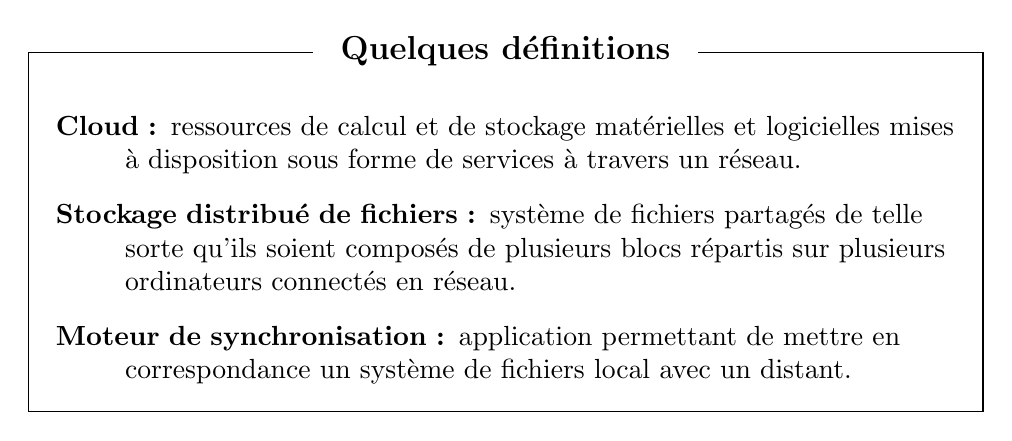
\begin{tikzpicture}
\node [text width=\textwidth - 20pt, draw, inner sep=10pt]
    (definitions) {
        \begin{description}
            \item[Cloud :] ressources de calcul et de stockage matérielles et logicielles mises à disposition sous forme de services à travers un réseau.
            \item[Stockage distribué de fichiers :] système de fichiers partagés de telle sorte qu'ils soient composés de plusieurs blocs répartis sur plusieurs ordinateurs connectés en réseau.
            \item[Moteur de synchronisation :] application permettant de mettre en correspondance un système de fichiers local avec un distant.
        \end{description}
    };
\node [fill=white, inner xsep=10pt] at (definitions.north)
    {\textbf{\large Quelques définitions}};
\end{tikzpicture}

Dans un premier temps, nous présenterons les méthodes et outils de travail que nous avons adoptés pour organiser ce projet. Ensuite, nous détaillerons la modélisation que nous avons choisie pour l'application, puis les technologies utilisées pour son implémentation. Enfin, nous ferons le point sur l'avancement du projet, les difficultés que nous avons rencontrées jusqu'ici et les perspectives qui s'offrent à nous pour la poursuite du développement d'Arcus.


% Sous-parties
\chapter{Organisation du projet}

\section{Méthode et organisation du travail}

Lors du développement d'Arcus, nous avons décidé de travailler un maximum de temps ensemble et de manière très régulière. Pour que nous puissions profiter tous deux des nombreuses connaissances que nous apporte le développement de ce projet, nous avons favorisé la méthode de programmation en binôme (ou \emph{pair programming}). Cette méthode consiste à donner la responsabilité de l'écriture du code à l'un des deux développeurs et à faire relire le code produit au fur et à mesure par le second développeur. Une étude menée par l'IEEE Computer Society~\parencite{mcdowell2003} a en effet montré que les étudiants utilisant cette méthode produisaient du code de meilleure qualité.

Afin d'être le plus efficace et d'avancer le plus rapidement possible nous nous sommes réunis quotidiennement. Durant les jours de la semaine, nous nous sommes vus entre 16~h~30 et 19~h~30, afin de faire le point sur l'avancement du projet, de définir les objectifs du jour et de les réaliser. Enfin, chaque week-end, nous avons réalisé les tâches en attente que nous n'avions pas pu faire durant la semaine.

Toutes les deux semaines, nous nous sommes réunis avec notre encadrante Mme~Hinde~Bouziane afin de faire le point sur l'état d'avancement de l'application. Cette réunion bihebdomadaire nous a également permis de bénéficier des ses conseils et de son aide sur les difficultés que nous avons rencontrées lors du développement.

\section{Répartition du travail dans le temps}

Nous avons découpé le développement du projet Arcus en deux périodes de temps. La première s'inscrit dans le cadre du T.E.R., et s'est déroulée de janvier à mi-mai 2017. La seconde aura lieu pendant un stage au Laboratoire d'Informatique, de Robotique et de Microélectronique de Montpellier (Lirmm) encadré par Mme~Hinde~Bouziane de fin-mai à fin-juin 2017. Par ailleurs, nous avons déjà effectué une semaine de stage au laboratoire au cours de la première semaine des vacances de printemps.

\clearpage

% Nous avons défini des objectifs pour chacune de ces différentes périodes.
Le but de la première période est d'obtenir une première version fonctionnelle de l'application qui répond à une partie du cahier des charges : la mise en place d'une interface commune aux différents services de stockage, la répartition des données de l'utilisateur sur ces services, leur réplication et le fonctionnement en tâche de fond.
% Au cours de la seconde période, nous finaliserons l'application en apportant les fonctionnalités manquantes : le chiffrement des données, le portage de l'application sur d'autres systèmes d'exploitation et une interface graphique pour l'application.

Ce rapport rend compte de notre avancement au cours de la première partie, c'est-à-dire pendant le projet T.E.R. Nous avons découpé cette période de travail en plusieurs phases.

\begin{enumerate}[label=\textbf{\arabic*.}]
    \item \textbf{Préparation du projet.} Nous avons écrit le cahier des charges de l'application, choisi les outils de travail et les principales technologies utilisées. Nous avons fait une première version du diagramme de répartition des tâches dans le temps, et une première modélisation de l'architecture de l'application.
    \item \textbf{Développement du projet.} Nous avons implanté les fonctionnalités de l'application en raffinant la modélisation au fur et à mesure. Pour chaque module implanté, nous nous sommes efforcés d'écrire des tests afin de s'assurer de leur bon fonctionnement.
    \item \textbf{Finalisation du projet.} Cette phase a consisté en la correction de bogues afin d'obtenir une version suffisamment stable pour pouvoir être présentée en vue de la soutenance et du rendu du projet T.E.R.
\end{enumerate}

L'annexe ~\ref{appendix:gantt} détaille cette répartition sous forme d'un diagramme de Gantt.

\section{Outils de travail collaboratif}

Nous avons choisi d'utiliser Git\footnote{Git : \url{https://git-scm.com/}} au travers du serveur GitLab\footnote{GitLab : \url{https://gitlab.info-ufr.univ-montp2.fr/matteodelabre/arcus/}} hébergé par le Service Informatique de la Faculté (Sif). Le logiciel Git, libre, permet la gestion des versions du projet et facilite la collaboration entre nous, notamment lorsque nous travaillions en même temps sur deux machines différentes. Les serveurs GitLab sont quant à eux basés sur un logiciel libre également et le service est fourni gratuitement par le Sif.

Pour communiquer entre nous à distance, nous avons utilisé Telegram\footnote{Telegram : \url{https://telegram.org/}} pour les messages écrits et appear.in\footnote{appear.in : \url{https://appear.in/}} pour la communication orale et le partage d'écrans.

Pour prendre des notes pendant les réunions, nous avons utilisé le langage Markdown\footnote{Markdown : \url{https://daringfireball.net/projects/markdown/}} qui permet un formattage rapide. Pour rédiger les différents documents, y compris ce rapport, nous avons utilisé \LaTeX\footnote{\LaTeX : \url{https://www.latex-project.org/}} pour sa capacité à produire des documents de bonne qualité.

Enfin, pour éditer le code du projet et les documents, nous nous sommes servis de l'éditeur de texte Atom\footnote{Atom : \url{https://atom.io/}}, logiciel libre développé par GitHub. Il s'agit en effet de l'éditeur que nous utilisons habituellement.

\chapter{Conception d'Arcus}

\tikzset{
    module/.style={
        rectangle, draw,
        minimum height=1.5em
    }
}

Nous avons commencé par décider d'une architecture globale pour l'application. Cette architecture est résumée dans la vue d'ensemble en figure~\ref{fig:conception-vue-ensemble}.

\begin{figure}[h!]
    \centering
    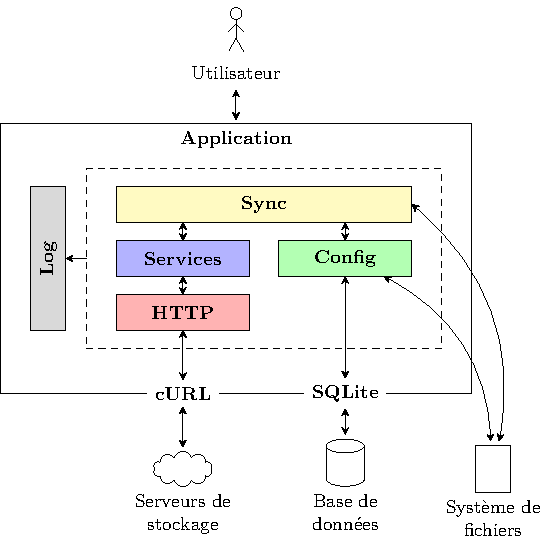
\includegraphics{figures/overview}
    \caption{\textbf{Vue d'ensemble de l'architecture de l'application.} Au centre, dans le cadre «~Application~», sont présentés les différents modules participant à l'architecture de l'application. Le niveau d'abstraction des modules va en croissant vers le haut du schéma. Les flèches représentent les interactions internes à l'application et celles entre les acteurs et ressources externes et l'application.}
    \label{fig:conception-vue-ensemble}
\end{figure}
\clearpage

Notre application a besoin de communiquer avec les interfaces de programmation (ou A.P.I.) des différents services de stockage de fichiers. Ces services fournissent en général une interface de communication utilisant \textit{HyperText Transfer Protocol} (HTTP). C'est un «~protocole applicatif pour les systèmes d'information distribués, collaboratifs utilisant des documents riches~»~\parencite{fielding1999}, donc particulièrement adapté au transfert de documents. Afin de communiquer avec ces services, notre application doit contenir un module de transmission de données sur HTTP, symbolisé par \tikz[baseline=(http.base)]\node[module,fill=red!30] (http) {\small{\textbf{HTTP}}}; dans la vue d'ensemble.

Bien que les fournisseurs de services de stockage connus tels que Nextcloud, OneDrive ou Dropbox utilisent HTTP, ils ont adopté des architectures hétérogènes qui font qu'il est difficile d'écrire un code unique permettant de communiquer avec toutes leurs interfaces. Dans notre application, nous devons donc construire une couche d'abstraction de ces hétérogénéités. Ce module, symbolisé par \tikz[baseline=(service.base)]\node[module,fill=blue!30] (service) {\small{\textbf{Services}}}; dans la vue d'ensemble, s'appuie sur les fonctionnalités du module HTTP.

Comme chaque utilisateur de la machine cliente peut choisir les répertoires qu'il souhaite synchroniser via l'application, la liste de ces répertoires doit être sauvegardée à un endroit de la machine. Ces informations sont regroupées dans une configuration dite locale spécifique à chaque utilisateur. Il existe par ailleurs des informations spécifiques à chaque répertoire synchronisé, comme par exemple la liste des fichiers présents ou la liste des services connectés. Ces informations sont quant à elles regroupées dans une configuration synchronisée sur les différentes machines d'un même utilisateur. Nous avons décidé d'isoler cette fonctionnalité dans un module de configuration, symbolisé par \tikz[baseline=(config.base)]\node[module,fill=green!30] (config) {\small{\textbf{Config}}}; dans la vue d'ensemble.

En s'appuyant sur ces différentes abstractions, nous pouvons mettre en place le moteur de synchronisation, cœur de l'application. Ce moteur doit permettre l'envoi des données contenues dans les répertoires sélectionnés par l'utilisateur vers les services de stockage connectés. Réciproquement, il doit permettre le rapatriement de celles-ci depuis les services distants vers la machine de l'utilisateur. Ce module est symbolisé par \tikz[baseline=(sync.base)]\node[module,fill=yellow!30] (sync) {\small{\textbf{Sync}}}; dans la vue d'ensemble.

Enfin, nous avons décidé qu'il était nécessaire de créer un module de journalisation. Grâce à ce module, les différents composants de l'application seront en mesure d'écrire des informations sur un journal global dans un format unifié. Ce journal global, qui pourra être redirigé vers la sortie standard ou un fichier, aidera au débogage en cas de défaillance de l'application. Dans la vue d'ensemble de l'architecture, il est symbolisé par  \tikz[baseline=(log.base)]\node[module,fill=gray!30] (log) {\small{\textbf{Log}}};.

\section{Transmission des données aux serveurs}

Le module HTTP permet l'échange de données entre un \emph{client} et un \emph{serveur} suivant le protocole HTTP. Ce protocole permet au client d'envoyer des demandes de données au serveur et de recevoir des réponses, mais pas l'inverse : c'est toujours le client qui demande des données au serveur. Pour ce faire, le client formule une requête, composée notamment d'un verbe, d'une \emph{Uniform Resource Locator} (URL) et d'une liste d'en-têtes. Le verbe spécifie l'action qui doit être entreprise sur la ressource désignée par l'URL. Les en-têtes servent à donner plus de détails sur la requête. La norme HTTP/1.1~\parencite{fielding1999} définit les verbes principaux suivants :

\begin{description}
    \item[\texttt{GET} :] récupérer les données contenues dans la ressource désignée par l'URL ;
    \item[\texttt{HEAD} :] récupérer les caractéristiques associées à la ressource désignée par l'URL ;
    \item[\texttt{POST} :] envoyer des données au serveur ;
    \item[\texttt{PUT} :] créer une ressource à l'URL donnée ;
    \item[\texttt{DELETE} :] supprimer la ressource désignée par l'URL.
\end{description}

Une fois la requête formulée par le client dans le module Services, celle-ci est transmise au serveur choisi. Ce serveur doit à son tour formuler une réponse qui satisfait la requête du client et la lui retourner. Ce mode de fonctionnement nous a amené à choisir la modélisation présentée dans la figure~\ref{fig:conception-http} pour le module HTTP.

\begin{figure}[h!]
    \centering
    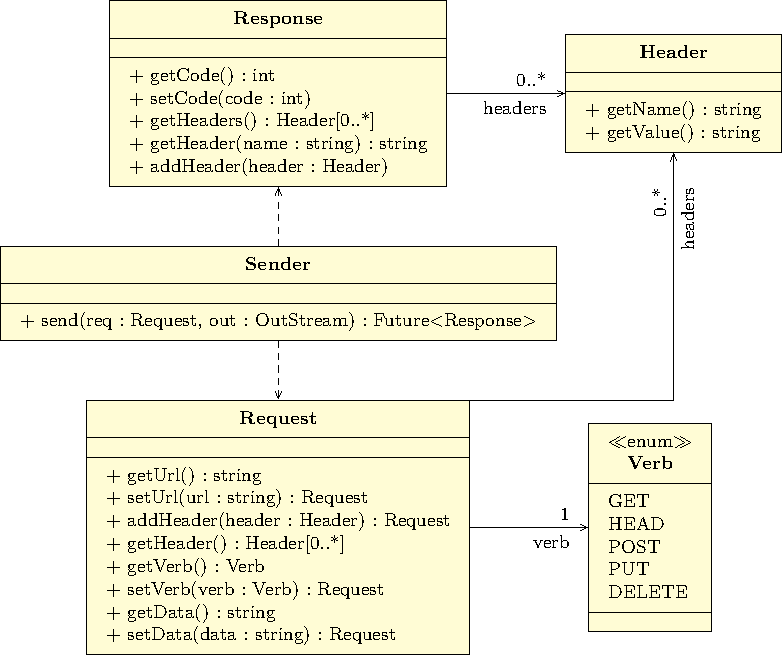
\includegraphics{figures/http}
    \caption{\textbf{Modélisation UML du module HTTP.} La classe \texttt{Sender} est au cœur du module, elle permet d'envoyer des requêtes et d'obtenir de façon asynchrone une réponse de la part du serveur. Cela signifie que le reste de l'application peut continuer à s'exécuter pendant que l'on attend la réponse du serveur à une demande. Ces requêtes doivent préalablement être construites selon le modèle donné par la classe \texttt{Request}. Les réponses fournies par le serveur suivent le modèle de la classe \texttt{Response}.}
    \label{fig:conception-http}
\end{figure}

\section{Définition d'une interface multi-services}

Le module Services a pour but d'abstraire le dialogue avec les interfaces de communication des différents services de stockage. Pour créer ce module, nous avons étudié les interfaces de deux fournisseurs de services majeurs : Dropbox et OneDrive. Nous avons constaté que chaque fournisseur avait une interface qui divergeait de celle de ses concurrents, faute de standard établi.

Par exemple, avec un compte OneDrive, pour obtenir des informations sur le quota alloué et son taux d'utilisation, il faut formuler une requête HTTP avec le verbe \texttt{GET} sur l'URL \url{https://graph.microsoft.com/v1.0/me/drive}~\parencite{onedrive-api}. À l'inverse, avec un compte Dropbox, pour obtenir les mêmes informations, la requête doit utiliser le verbe \texttt{POST} et porter sur l'URL \url{https://api.dropboxapi.com/2/users/get_space_usage}~\parencite{dropbox-api}.

Nous voyons sur ces exemples que les verbes HTTP ou les URL à utiliser pour accéder aux ressources sur les services sont variables.
Toutefois, parmi les services de stockage de fichiers les plus connus, une large majorité a adopté une architecture d'interface de communication dite en \emph{Representational State Transfer} (Rest). Ce type d'architecture, théorisée par \citeauthor{fielding2000} en \citeyear{fielding2000}, repose sur les principes suivants.

\begin{description}
    \item[\textbf{Utilisation sémantique de HTTP.}] L'interface utilise le protocole HTTP décrit dans le module précédent. Elle associe sémantiquement les verbes du protocole à chaque action réalisable ; par exemple, elle utilise le verbe \texttt{GET} lorsqu'il s'agit de récupérer des informations ou \texttt{DELETE} pour en supprimer. Elle utilise les URL pour désigner des ressources et non pas, par exemple, pour désigner une page de connexion.

    \item[\textbf{Échange de requêtes et réponses descriptives.}] Toutes les informations nécessaires au traitement d'une requête du client sont contenues uniquement dans celle-ci. Le serveur n'utilise pas d'informations contextuelles qui seraient liées aux requêtes précédemment effectuées. Il renvoie des réponses descriptives pouvant être traitées en tant que telles sans avoir besoin d'effectuer une requête supplémentaire.

    \item[\textbf{Exclusivité d'accès aux données via le serveur.}] Le serveur est le seul ayant accès à la base de données ou aux informations quelles qu'elles soient. Le client n'y accède que par l'intermédiaire du serveur. Cela simplifie notamment la gestion de la cohérence des données puisque seul le serveur en est responsable.
\end{description}

Les interfaces de OneDrive et Dropbox que nous avons étudiées s'efforcent de suivre ces principes, même s'il subsiste des incompatibilités. Nous avons décidé de profiter du fait que le protocole HTTP soit commun à une très grande majorité des interfaces de communication des services de stockage pour construire notre abstraction. Les incompatibilités nous ont amené à conclure qu'il serait très difficile d'écrire un code unique pour accéder aux différents services.

Nous avons donc créé une interface commune pour accéder à celles des services de stockage, puis réalisé différentes implémentations de cette interface, une par service supporté. Cette modélisation nous permettra d'intégrer plus facilement de nouveaux services par la suite sans devoir modifier le code des autres modules. La figure~\ref{fig:conception-services} présente l'architecture du module Services.

\begin{figure}[h!]
    \centering
    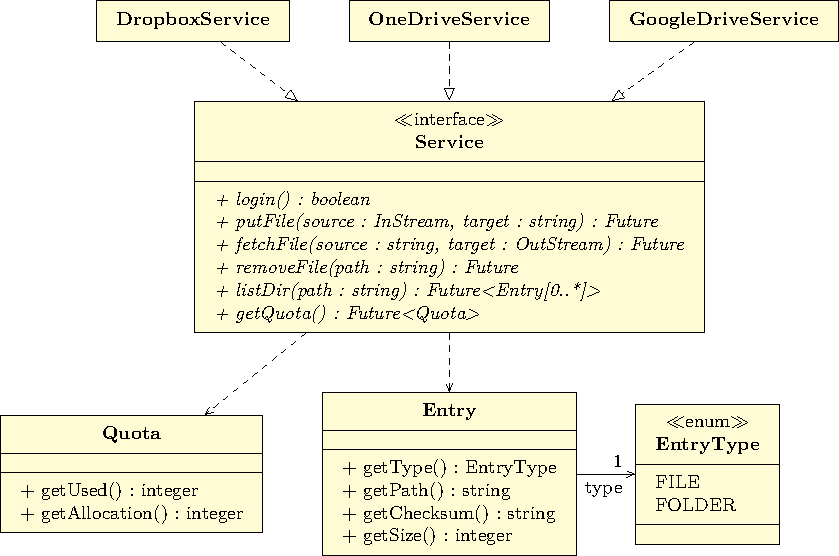
\includegraphics{figures/services}
    \caption{\textbf{Modélisation UML du module Services.} L'interface \texttt{Service} est l'élément principal du module. Elle définit les actions communes que l'application doit être en mesure de réaliser sur chaque service : authentification, ajout d'un fichier, récupération d'un fichier, suppression d'un fichier, listage d'un répertoire, récupération du quota et de son utilisation. Toutes ces actions sont asynchrones.}
    \label{fig:conception-services}
\end{figure}

\section{Configuration locale et configurations synchronisées}

\subsection{Notion de zone de synchronisation}

Nous avons décidé lors de la rédaction du cahier des charges de permettre à l'utilisateur de synchroniser les données d'un ensemble de répertoires (et de leurs sous-répertoires) de son choix. Nous désignerons dans la suite de ce rapport les données de chaque répertoire par l'expression «~zone de synchronisation~».

Ces zones sont associées à un unique répertoire sur la machine de l'utilisateur, situé n'importe où dans son répertoire d'accueil. Elles ne peuvent pas se chevaucher : aucun fichier n'appartient à deux zones de synchronisation.

Pour chaque zone, l'application doit être en mesure de reconstituer les fichiers dispersés en blocs sur les différents services. Pour ce faire, elle a besoin de conserver des informations sur la répartition de ces blocs. Elle a également besoin de pouvoir comparer l'état des zones de la machine actuelle avec celles du serveur, afin de réaliser la synchronisation.

En particulier, nous avons besoin pour chaque bloc de savoir de quel fichier il fait partie, l'ordre dans lequel il apparaît, les services de stockage sur lesquels il est stocké et peut être récupéré. Enfin, l'application a besoin de conserver les informations d'authentification pour chaque service.

\subsection{Conception d'un index d'état}

Pour répondre à ces besoins, nous avons choisi de mettre en place un index d'état pour chaque zone. Cet index est synchronisé avec chaque service de stockage utilisé, afin de pouvoir être récupéré par d'autres machines et servir de base à la reconstitution du répertoire associé. Il contient les informations sur les blocs, les fichiers et les services.

Chaque bloc fait partie d’un unique fichier et possède un identifiant unique indépendant de ce fichier. Il est stocké sur au moins un service. L'index stocke également le \emph{hash} du bloc, correspondant à une somme de contrôle des données qu’il contient, et permettant de savoir si ces données ont changé. Enfin, chaque bloc possède un numéro d’ordre qui indique la position qu’il occupe dans le fichier original relativement aux autres.

Chaque fichier et chaque répertoire possède un identifiant unique indépendant de son chemin. Nous avons décidé d'utiliser une structure récursive pour stocker l'arborescence de la zone de synchronisation, dans laquelle chaque fichier ou répertoire est lui-même fils d'un autre répertoire. Chaque fichier possède un nom et contient au moins un bloc.

Enfin, les comptes de services de stockage que l'utilisateur a connectés à la zone sont stockés dans l'index. Ces comptes contiennent un ensemble de blocs de fichiers synchronisés. L'application conserve le nom du fournisseur du service en question ainsi que les informations d'authentification. Dans cette première modélisation de l'application, nous conservons les informations d'authentification en clair dans l'index, nous ne tenons donc pas compte de leur sécurité. Nous réglerons ce problème dans le futur en chiffrant l'index.

En raison de la complexité de la structure de l'index, nous avons choisi de le stocker sous forme d'une base de données relationnelle, dont le modèle entité-association est présenté en figure~\ref{fig:conception-base}.

\begin{figure}[h!]
    \centering
    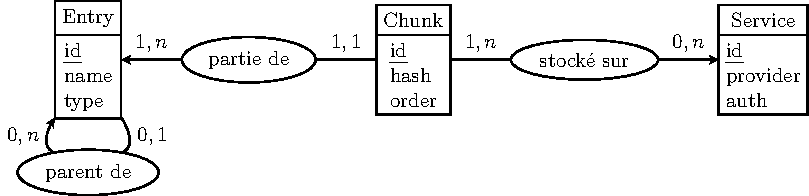
\includegraphics{figures/base}
    \caption[Modèle entité-association de la base de données de l'index]{\textbf{Modèle entité-association de la base de données pour l'index.}}
    \label{fig:conception-base}
\end{figure}

De ce fait, nous avons choisi de considérer chaque zone de synchronisation comme une entité totalement indépendante, possédant sa propre configuration synchronisée avec différents services, sous forme d'une base de données.

Sur cet aspect, notre conception s'apparente à celle du logiciel Git qui définit des \emph{dépôts}, semblables à nos zones de synchronisation, qui contiennent leur propre index~\parencite{rosenberg2010} et sont synchronisés avec un serveur distant. Nous divergeons cependant sur le fait que Git se concentre sur l'aspect de gestion de versions des données, ce que notre application ne prend pas en compte car cela ne correspond pas aux objectifs que nous nous sommes fixés.

Ce choix permet une plus grande flexibilité pour l'utilisateur. En effet, si nous avions choisi de centraliser le stockage des informations d'authentification des services de toutes les zones de synchronisation dans un seul fichier, il n'aurait par exemple pas été possible de synchroniser une zone avec deux services particuliers et une autre avec deux différents.

En choisissant de stocker le plus d'informations possible dans une configuration spécifique à chaque zone, l'application peut non seulement fonctionner dans le cas où ces zones ne partagent pas les mêmes services, mais également dans le cas où elles les partagent.

\subsection{Conception d'une configuration locale}

Comme expliqué avant, les zones de synchronisation sont associées, sur une machine, à un répertoire racine. Si l'on synchronise cette zone avec une autre machine, il y a de fortes chances pour que l'on souhaite l'associer à un répertoire ayant un chemin différent. Par exemple, le nom de l'utilisateur peut avoir changé entre les deux machines, ou elles peuvent ne pas fonctionner sur le même système d'exploitation.~\footnote{Le système Windows place par exemple le répertoire d'accueil de l'utilisateur dans \texttt{C:\textbackslash{}Users\textbackslash{}utilisateur} alors que les dérivés de GNU/Linux utilisent généralement \texttt{/home/utilisateur}.}

Pour gérer ces cas, nous avons décidé de créer un fichier de configuration local sur chaque machine et pour chaque utilisateur. Ce fichier contient les paramètres qui n'ont pas lieu d'être partagés par plusieurs machines.

Dans cette configuration, pour le moment seule la liste des associations entre chaque zone de synchronisation et son répertoire racine pour la machine actuelle est stockée. Nous pourrons y inclure plus de paramètres si le besoin se présente dans le futur. La figure~\ref{fig:conception-syncdir} montre un exemple de mise en place de ces différentes configurations sur un système GNU/Linux.

\begin{figure}[h!]
    \centering
    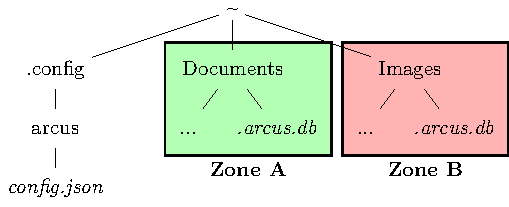
\includegraphics{figures/syncdir}
    \caption{\textbf{Exemple de répartition des différentes configurations de l'application.} Les fichiers dont le nom est en italique contiennent les configurations de l'application telles que décrites dans les parties précédentes. La configuration locale, unique pour l'utilisateur, est stockée dans \texttt{\textasciitilde{}/.config/arcus/config.json}. Dans cet exemple, l'utilisateur a choisi de synchroniser deux zones, A associée aux répertoire des documents et B associée aux répertoire images. Dans chacune de ces zones, la base de données est stockée dans le fichier \texttt{.arcus.db}.}
    \label{fig:conception-syncdir}
\end{figure}

\subsection{Gestion des configurations dans l'application}

Notre application doit ainsi gérer deux configurations, une configuration synchronisée spécifique à chaque zone, et une configuration locale pour chaque utilisateur, qui est dépendante de la machine utilisée. Pour ce faire, nous avons conçu un module de configuration dont la modélisation est présentée en figure~\ref{fig:conception-config}.

\begin{figure}[h!]
    \centering
    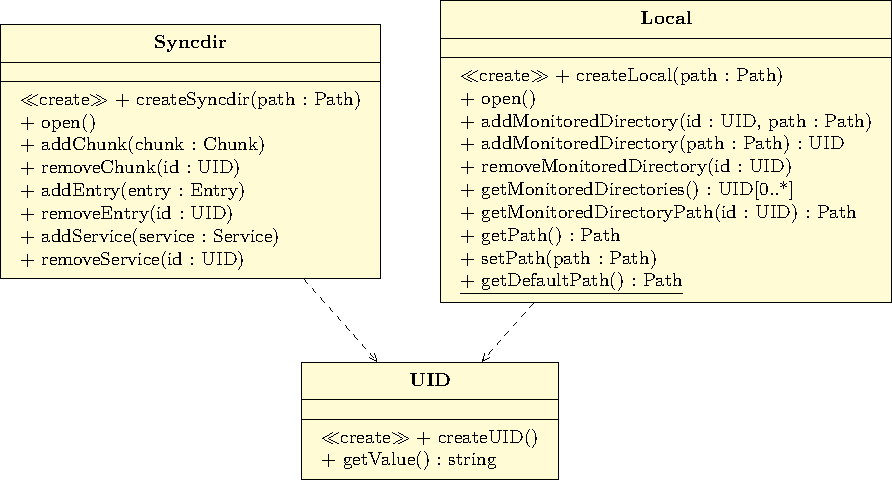
\includegraphics{figures/config}
    \caption{\textbf{Modélisation UML du module Config.} La classe \texttt{Local} permet la lecture et l'écriture de la configuration locale et la gestion des associations entre les zones de synchronisation et leur répertoire. La classe \texttt{Syncdir} permet de gérer la base de données associée à une zone particulière. Enfin, la classe \texttt{UID} permet la génération d'identifiants uniques, utilisés pour identifier les fichiers, les zones de synchronisation, les blocs et les services.}
    \label{fig:conception-config}
\end{figure}

\section{Moteur de synchronisation des fichiers}

Le moteur de synchronisation constitue la partie principale de l'application. Il s'appuie sur les fonctionnalités et les abstractions construites dans les modules précédents. Son rôle est de s'assurer que les zones de synchronisation locales et sur le serveur restent synchronisées.

Pour ce faire, il observe les changements effectués par l'utilisateur dans les zones de synchronisation locales à sa machine. À chaque changement local, il téléverse les données vers les serveurs distants en les répartissant. Réciproquement, à chaque changement distant, il télécharge les données et reconstitue les fichiers en local.

Lors de cette procédure de synchronisation, nous distinguons trois cas qui peuvent se présenter.

\begin{description}
    \item[Modification locale sans modification distante.] Ce cas est le plus courant. Il se produit lorsque des changements locaux sont effectués sur une machine et qu'aucune modification n'est effectuée entre temps sur les serveurs.

    \item[Modification distante sans modification locale.] Ce cas ne peut se produire que lorsqu'au moins deux machines sont synchronisées avec les mêmes serveurs. Par exemple, si un utilisateur effectue des changements sur une machine B et les envoie sur les serveurs, et qu'aucune modification n'est effectuée sur une machine A. Alors, dans le référentiel de la machine A, il y a eu des changements distants sans modification locale.

    \item[Modification locale et distante.] Ce cas est le plus problématique, et ne peut se produire que lorsqu'au moins deux machines sont synchronisées avec les mêmes serveurs. Par exemple, si un utilisateur effectue des changements sur une machine A et une machine B, que les changements de la machine B sont envoyés en premier et que la machine A cherche à se synchroniser. Alors, dans ce cas, dans le référentiel de la machine A, il y a eu des changements distants et des changements locaux, il y a donc conflit.
\end{description}

Chacun de ces trois cas doit être traité par une procédure différente. Le moteur doit donc être en mesure de distinguer les trois cas afin d'enclencher la bonne procédure.

Pour discriminer ces cas, nous avons choisi d'utiliser un numéro de version, stocké dans la base de données de chaque zone. Ce numéro est fixé à 0 initialement. À chaque modification ce numéro est incrémenté, avant d'envoyer les changements vers le serveur. Un algorithme permettant de discriminer les trois cas en utilisant le numéro de version est présenté dans la figure~\ref{fig:conception-sync-discr}.

\begin{figure}[h]
    \centering
    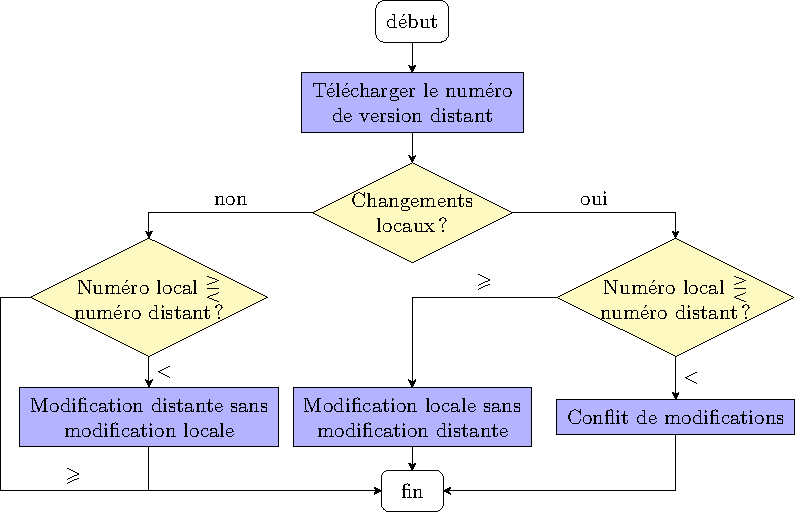
\includegraphics{figures/sync-discr}
    \caption{\textbf{Algorithme de discrimination des différents cas de synchronisation.} Dans le cas où il y a des changements locaux, alors, si le numéro local est strictement inférieur au numéro distant, on se trouve dans le cas où il y a des modifications locales sans modification distante. Sinon, il y a un conflit de modifications. À l'inverse, s'il n'y a pas de modificaiton locale, alors il y a des modifications distantes seulement si le numéro local est strictement inférieur au numéro  distant. Sinon, il n'y a rien à faire.}
    \label{fig:conception-sync-discr}
\end{figure}

Cependant, il persiste un cas ambigu : si le numéro de version distant est incrémenté entre le moment où nous le téléchargeons depuis le serveur et le moment où nous le comparons dans l'algorithme. Dans la version initiale d'Arcus, nous avons décidé de ne pas traiter ce cas pour simplifier le traitement, mais nous le traiterons toutefois dans le futur.

\section{Journal des actions de l'application}

Comme nous l'avons détaillé précédemment, l'application est responsable de la synchronisation de plusieurs répertoires, d'échanges de données avec des serveurs, de la gestion de configurations... Ces fonctionnalités sont souvent complexes, et nous avons anticipé le fait que lorsque des bogues se produiront à l'exécution, ils seront éventuellement difficiles à résoudre.

Pour pallier ce problème, nous avons décidé de créer un journal des actions de l'application. Celui-ci permet de retranscrire précisément la séquence d'actions effectuée par l'application, d'identifier plus facilement les problèmes éventuels et de remonter à la source de ceux-ci.

Nous avons pour cela décidé d'associer à chaque message du journal la date et l'heure à laquelle il a été produit. Cette date est formattée en ISO 8601~\parencite{iso8601} pour éviter toute ambiguïté et faciliter son interprétation par d'autres applications. Nous avons attribué à chaque message un niveau de sévérité (informatif, avertissement ou erreur) et un code couleur qui permettent de relever facilement les informations importantes. Enfin, la ligne de code ayant produit un message lui est clairement associée afin de pouvoir diagnostiquer plus facilement les éventuels problèmes. La figure~\ref{fig:conception-journal} résume le format que nous avons choisi pour les messages du journal.

\begin{figure}[h!]
    \centering
    
\begin{tikzpicture}[font=\ttfamily, node distance=0cm]
        \node (date-heure)
            {\textcolor{black!70}{YYYY-MM-DD}T\textcolor{black!70}{HH:MM:SS}};

        \node[right=of date-heure] (niveau)
            {[\textcolor{green!80!black}{info}|\textcolor{orange!80!black}{warn}|\textcolor{red!80!black}{err!}]};

        \node[right=of niveau] (source)
            {\textcolor{black!70}{fichier}:\textcolor{black!70}{ligne}};

        \node[right=of source] (sep) { - };

        \node[right=of sep] (message)
            {\textcolor{black!70}{Message}};

        \tikzset{font=\rmfamily\itshape}

        \node[below=of date-heure] {Date et heure};
        \node[below=of niveau] {Sévérité};
        \node[below=of source] {Source};
    \end{tikzpicture}

    \caption{\textbf{Format unifié d'écriture des messages pour le journal de l'application.}}
    \label{fig:conception-journal}
\end{figure}

\chapter{Implémentation d'Arcus}

Nous avons choisi de développer le projet Arcus en C++. En effet, le C++ est un langage orienté objet, ce qui correspond à la modélisation objet que nous avons réalisé pour notre application, et multi-plateformes, ce qui nous permettra de porter l'application sur plusieurs systèmes relativement facilement.

Par ailleurs, le C++ est l'un des principaux langages enseignés dans notre formation. Nous possédons donc des acquis avec ce langage, et ce projet nous permet d'en améliorer notre connaissances. Enfin, ce langage jouit d'une communauté importante, de nombreuses bibliothèques ainsi que d'une documentation très complète.

Nous avons choisi d'utiliser C++11, la version de C++ spécifiée par le standard publié en 2012~\parencite{cpp11}. Celle-ci ajoute de nombreuses fonctionnalités au langage et à la bibliothèque standard, entre autres le multi-tâches, les lambdas, les tables de hachage et les expressions régulières.

Nous compilons notre code avec le compilateur Clang, et, pour automatiser la compilation, nous avons utilisé CMake. CMake dispose d'un méta-langage qui permet de produire à la fois des fichiers pour Make, XCode, Visual Studio et d'autres environnements. Il facilite donc le portage.

Ces choix sont résumés dans la table~\ref{table:implementation-tools}.

\section{Mise en place de la communication avec les serveurs}

Pour réaliser le module de communication, nous avons décidé d'utiliser la bibliothèque cURL.\footnote{cURL : \url{https://curl.haxx.se/}} L'utilisation de cette bibliothèque nous permet de bénéficier de sa robustesse, sa simplicité et sa fiabilité. Il s'agit par ailleurs d'une des bibliothèques les plus utilisées pour la communication sur HTTP, notamment utilisée par Adobe, Apple, Microsoft, Mozilla et Spotify~\parencite{curl-companies}. La plupart des problèmes que nous pouvons rencontrer avec cette bibliothèque sont donc déjà documentés.

Nous avons opté pour une implémentation permettant de traiter les requêtes en provenance du module Services de manière asynchrone. Le but est que, pendant l'envoi d'une requête et l'attente de sa réponse, le module puisse continuer d'accepter d'autres requêtes de la part de l'application. Ainsi l'application peut continuer à s'exécuter en attendant le téléversement ou le téléchargement de données vers ou depuis un serveur.

Pour ce faire, nous avons réalisé une implémentation multi-tâches avec deux tâches parallèles : une tâche principale qui reçoit les requêtes et une tâche qui s'occupe de les envoyer et de réceptionner les réponses. Cette implémentation exploite les fonctionnalités de multi-tâches introduites en C++11, en complément de la bibliothèque Boost Thread.~\footnote{Boost Thread : \url{http://www.boost.org/doc/libs/1_64_0/doc/html/thread.html}}

Lorsque la tâche principale reçoit une requête en provenance du module Service, elle l'ajoute dans une file d'attente des requêtes à envoyer et continue son exécution. En parallèle, la tâche d'envoi et de réception boucle en permanence en attendant que des requêtes arrivent dans la file d'attente. Elle les envoie alors une par une aux serveurs distants et réceptionne les réponses. Lorsqu'une réponse est reçue par la tâche d'envoi et de réception, celle-ci est transmise à la tâche principale via une promesse. La figure~\ref{fig:implementation-http-thread}, donne un exemple de comportement de ces deux tâches.

\begin{figure}[h]
    \centering
    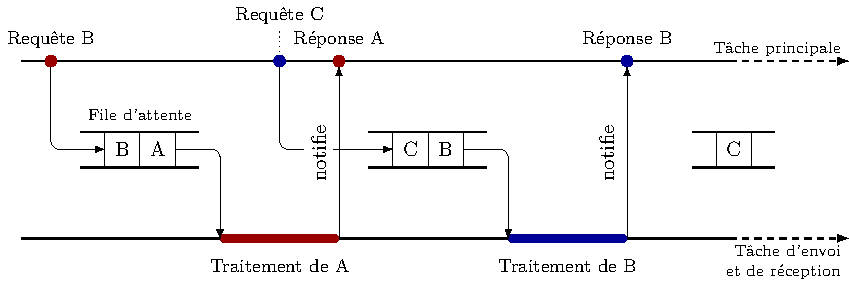
\includegraphics{figures/implementation-thread}
    \caption{\textbf{Exemple de comportement des deux tâches lors d'envois de requêtes.} La tâche principale reçoit une requête supplémentaire C pendant que la tâche d'envoi et de réception est en train de traiter la requête A.}
    \label{fig:implementation-http-thread}
\end{figure}

À chaque envoi de requête, la bibliothèque cURL ouvre une nouvelle connexion au serveur demandé. Ce comportement peut se révéler inefficace notamment si plusieurs requêtes vers le même serveur sont envoyées à la suite. Pour limiter ce problème, nous avons créé une classe de piscine~\emph{(pool)} permettant de mutualiser les ressources et notamment de garder la même connexion ouverte pour plusieurs requêtes vers le même serveur dans un intervalle de temps court.

L'annexe~\ref{appendix:code-sender} présente les principaux extraits du code gérant la synchronisation entre les deux tâches et l'utilisation de la bibliothèque cURL. La figure~\ref{fig:implementation-http-exemple} montre un exemple d'utilisation du module comme il pourrait l'être dans le module Services.

\begin{figure}[h!]
    \begin{lstlisting}[language=C++]
HTTP::Request req = HTTP::Request()
    .setUrl("https://fr.wikipedia.org/wiki/Wikip%C3%A9dia:Accueil_principal")
    .setVerb(HTTP::Verb::GET);

HTTP::Sender sender;
sender.send(req, &std::cout).get();
    \end{lstlisting}
    \caption{\textbf{Exemple d'utilisation du module HTTP pour envoyer une requête.} Dans cet exemple, le contenu de la page d'accueil de Wikipédia est téléchargé et affiché la sortie standard. Grâce au travail réalisé dans ce module, nous sommes en mesure d'écrire un code concis de haut niveau pour envoyer des requêtes HTTP et récupérer leur réponse.}
    \label{fig:implementation-http-exemple}
\end{figure}

\section{Création de l'interface commune aux services}

L'objectif du module Services est de fournir une abstraction de la communication avec les interfaces des services de stockage. Pour fournir cette abstraction, nous avons implémenté une classe pour chaque service de stockage. Chacune de ces classes réalise l'interface présentée dans la partie conception.

Dans ces classes, chaque action abstraite requise par l'interface, comme l'ajout d'un fichier ou la récupération du quota, est «~traduite~» en une requête ou série de requêtes permettant de réaliser cette action sur le service. Une fois la réponse du serveur du service reçue, celle-ci est transformée dans les structures de données utilisées par notre application.

L'implémentation de ce module ne présente pas de complexité technique particulière, si ce n'est celle de manier correctement le concept de promesses. Cette simplicité est due au fait que les détails d'implémentation de la communication sont cachés dans le module HTTP. L'annexe~\ref{appendix:code-service} montre quelques exemples de traduction des actions pour l'A.P.I. de Dropbox.

Vu de l'extérieur de ce module, la communication avec l'un ou l'autre des services supportés est totalement transparente. Cela nous permet, dans les autres modules, de manipuler un service de façon abstraite sans craindre de devoir modifier le code en cas d'ajout d'un nouveau service.

\section{Formats de stockage des configurations}

Nous avons choisi, pour stocker la configuration synchronisée, une base de données SQLite~3.\footnote{SQLite~3 : \url{https://www.sqlite.org/}} Nous avons donc converti notre modèle entité-association, présenté dans la partie conception, en modèle relationnel, décrit dans la figure~\ref{fig:implementation-config-bd}. Nous avons choisi la bibliothèque SQLite~3 car elle dispose d'une A.P.I. simple d'utilisation, et que les bases de données produites sont contenues dans un unique fichier, ce qui simplifie grandement leur synchronisation avec les différents services.

\begin{figure}[h]
    \begin{lstlisting}[escapeinside={(*}{*)}]
Entry((*\uline{id}*), name, type, (*\dashuline{parent}*))
Chunk((*\uline{id}*), hash, order, (*\dashuline{File.id}*))
ChunkService((*\dashuline{Chunk.id}*), (*\dashuline{Service.id}*))
Service((*\uline{id}*), provider, auth)
    \end{lstlisting}
    \caption{\textbf{Modèle relationnel de la base de données.}}
    \label{fig:implementation-config-bd}
\end{figure}

En raison de la simplicité de la structure de la configuration locale de notre application, nous avons choisi un format plus léger qu'une base de données : le \emph{JavaScript Object Notation} (JSON, \cite{ecma404}). Ce format a l'avantage d'être simple et compréhensible par un humain. Pour lire et écrire les fichiers JSON, nous utilisons la bibliothèque \texttt{nlohmann::json}\footnote{\texttt{nlohmann::json} : \url{https://github.com/nlohmann/json}}. La figure~\ref{fig:conception-local} présente le format de ce fichier.

\begin{figure}[h]
    \begin{verbatim}{
    "monitored_directories": {
        "ID-ZONE-1": "/chemin/zone-1/",
        "ID-ZONE-2": "/chemin/zone-2/",
        "ID-ZONE-3": "/chemin/zone-3/"
    }
}\end{verbatim}
    \caption{\textbf{Format du fichier de configuration local.} Sous la clef \texttt{monitored\_directories} se trouve un dictionnaire associant les identifiants des zones de synchronisation aux chemins des répertoires sur lesquels elles sont attachées.}
    \label{fig:conception-local}
\end{figure}

Pour les identifiants dans les fichiers de configuration, nous utilisons des \emph{Universally Unique IDentifier} (UUID). Pour les générer, nous utilisons la bibliothèque Boost UUID~\footnote{Boost UUID : \url{http://www.boost.org/doc/libs/1_64_0/libs/uuid/uuid.html}} qui est compatible avec la majorité des systèmes d'exploitation.

\section{Détection des changements dans le système de fichiers}

Afin de détecter l'ajout, la suppression ou la mise à jour des fichiers locaux, nous utilisons fswatch\footnote{\texttt{fswatch} : \url{http://emcrisostomo.github.io/fswatch/}}. Cette bibliothèque a le grand avantage d'abstraire derrière une A.P.I. C++ de haut niveau les mécanismes très divers des différents systèmes d'exploitation permettant l'observation des changements effectués dans le système de fichiers. Son utilisation permettra d'adapter Arcus sur plusieurs systèmes plus facilement.

\begin{table}[h]
    \centering
    \begin{tabular}{lll}
        & \textbf{Fonction} & \textbf{Outil}\\
        \toprule
        \textbf{Code} & Langage & C++11\\
        \cmidrule{2-3}
        & Compilateur & Clang\\
        \cmidrule{2-3}
        & Construction automatisée & CMake\\
        \midrule
        \textbf{Bibliothèques} & Requêtes HTTP & cURL\\
        \cmidrule{2-3}
        & Base de données & SQLite~3\\
        \cmidrule{2-3}
        & Interprétation JSON & \texttt{nlohmann::json}\\
        \cmidrule{2-3}
        & Observation arborescence & fswatch\\
        \cmidrule{2-3}
        & Chemins et système de fichiers & Boost Filesystem\\
        \cmidrule{2-3}
        & Identifiants uniques & Boost UUID\\
        \cmidrule{2-3}
        & Threads & Bibliothèque standard et Boost Thread\\
        \bottomrule
    \end{tabular}

    \caption{\textbf{Résumé des technologies choisies pour l'implémentation.}}
    \label{table:implementation-tools}
\end{table}

\chapter{Bilan et difficultés rencontrées}

\section{Bilan de l'avancement du projet}

Nous avons terminé l'implémentation du module de communication via HTTP. Pour tester ce module, nous avons développé un programme de test effectuant des échanges avec le serveur \url{www.example.com} sur différents types de requêtes. Nous nous sommes ainsi assurés du bon fonctionnement de ce module, y compris lorsque plusieurs requêtes sont envoyées en parallèle. Désormais, le module est utilisable pour l'envoi de requêtes avec n'importe quel verbe sur n'importe quelle URL.

Nous avons également fini la création du module des services, et créé une classe permettant d'utiliser le service de stockage Dropbox. Nous avons écrit un programme de test qui récupère le quota, liste un répertoire, envoie des fichiers et en supprime sur un compte Dropbox. Ce test permet également de valider le bon fonctionnement du module HTTP qui est utilisé par la classe.

À l'heure où nous écrivons ces lignes, Arcus est capable de communiquer avec Dropbox. Nous travaillons actuellement sur l'intégration de OneDrive, le service de Microsoft, que nous comptons terminer pour le rendu du livrable. Ce travail permettra de montrer la facilité avec laquelle un nouveau service peut être intégré dans l'interface multi-services, et ce sans aucune modification dans les autres modules.

Nous avons achevé la réalisation du module de journalisation des actions de l'application, et celui-ci est utilisé à travers les autres modules. Nous avons également développé un programme pour tester la création du journal et la cohérence des messages affichés.

Nous avons aussi terminé la mise en place du module permettant de manipuler les configurations locales et distantes, y compris l'intégration avec la bibliothèque de lecture et d'écriture du JSON et SQLite~3. Nous avons vérifié que le comportement de ce module soit correct avec un programme de tests écrivant et lisant des configurations locales et créant des bases de données.

Enfin, au moment de la rédaction de ce rapport, nous sommes en train de finaliser le moteur de synchronisation afin de faire fonctionner notre application. Nous prévoyons de finaliser ce dernier module dans les semaines à venir.

Sur les modules que nous avons mis en place et testés, nous nous sommes efforcés de régler tous les bogues que nous avons pu rencontrer, et nous n'avons pas pour le moment connaissance des éventuels bogues restants.

\section{Difficultés rencontrées}

La conception de notre application a été une première difficulté. En effet, nous n'avions encore jamais travaillé sur la conception d'une application de cette taille. Nous avons donc passé plusieurs semaines à définir le cahier des charges et les modèles afin d'éviter de nous bloquer par la suite en poursuivant avec un modèle erroné. Nous les avons ensuite raffinés pendant la phase d'implémentation.

Au cours de la création du module HTTP de notre application, nous avons été confrontés pour la première fois à la programmation concurrente. Nous avons donc dû apprendre les concepts liés à ce type de programmation, tels que les tâches, les méthodes de synchronisation de ces tâches, les promesses et valeurs futures. Nous avons rapidement rencontré les problèmes couramment associés aux tâches et à leur synchronisation, tels que les \emph{deadlocks} ou les \emph{race conditions}. Ce nouvel apprentissage a constitué pour nous une difficulté importante, et nous sommes parvenus à la surmonter grâce à l'aide de notre encadrante.


% Conclusion
\chapter*{Conclusion et perspectives}
\addcontentsline{toc}{chapter}{Conclusion et perspectives}

\section*{Connaissances et apprentissages}

Ce projet nous a permis de mettre en pratique et de consolider de nombreuses connaissances aquises tout au long de notre parcours universitaire. Nous donnons dans cette partie des exemples d'enseignements qui nous ont été utiles dans la réalisation de ce projet.

L'enseignement en systèmes d'information et bases de données~(HLIN304) nous a appris a concevoir une base de données, à la gérer et à l'interroger avec le langage SQL. Cela nous a permis de concevoir la base de données de notre application.

Nous avons appris à programmer en C++ à l'aide des enseignements de programmation impérative~(HLIN202, HLIN302). Nous avons pu utiliser la programmation orientée objet et modéliser nos modules en UML grâce aux cours de modélisation et de programmation par objet~(HLIN406).

Les cours de techniques de communication, de conduite de projets~(HLIN408) et de projet C.M.I.~(HLSE205) nous ont fait découvrir la gestion de projet et permis d'apprendre à utiliser de nombreux outils utiles tels que \LaTeX, Git, GitLab, Make et gdb...

Enfin, nous avons découvert et appris à nous servir du format JSON avec l'enseignement «~du binaire au web~»~(HLIN102).

Ce projet nous a également permis de développer de nouvelles compétences. En particulier, tout ce qui concerne le réseau a été une découverte pour nous. Nous avons appris les principes de HTTP, exploré l'A.P.I. Rest fournie par Dropbox et OneDrive et étudié le fonctionnement de la bibliothèque cURL. Nous avons également appris les bases de la programmation concurrente.

Enfin, ce projet a été l'occasion de découvrir le fonctionnement et l'interface de SQLite~3. Il nous a permis de voir une première utilisation concrète des bases de données.

\section*{Perspectives}

La seconde partie de notre projet, que nous réaliserons en stage au laboratoire d'informatique, de robotique et de microélectronique de Montpellier (Lirmm) entre le 30~mai et le 30~juin, sera l'occasion d'implémenter les fonctionnalités encore manquantes à notre application.

Nous nous occuperons de la sécurité de l'application, notamment du chiffrage des informations d'authentification et des données de l'utilisateur. Nous doterons également notre application d'une interface graphique simple permettant de faciliter sa configuration. Nous prévoyons également de porter notre application sur plusieurs systèmes. Enfin, nous prévoyons d'intégrer notre application avec plus de services.


% Annexes
\renewcommand{\appendixpagename}{Annexes}
\renewcommand{\appendixtocname}{Annexes}

\begin{appendices}
    \documentclass[tikz]{standalone}

\usepackage[utf8]{inputenc}
\usepackage[T1]{fontenc}
\usepackage{lmodern}

\usepackage[french]{babel}
\usepackage[french]{translator}
\usepackage{textcomp}
\usepackage{pgfgantt}

\usetikzlibrary{babel}

\ganttset{
    % Format de la date en YYYY-MM-DD
    time slot format=isodate,
    %
    % Traduction des étiquettes en français
    today label={\textbf{Aujourd’hui}\\5 mai 2017},
    calendar week text={Semaine~\currentweek},
    %
    % Grille verticale tous les 7 jours
    vgrid={*6{draw=none},{dotted}},
    %
    % Positionnement des étiquettes des tâches
    inline,
    milestone inline label node/.append style={left=2.5mm},
    link label node/.append style={anchor=east},
    %
    % Affichage du jour actuel dans le diagramme
    today={2017-05-05},
    today label node/.append style={align=center}
}

\setganttlinklabel{f-s}{fin à début}
\setganttlinklabel{f-f}{fin à fin}

\begin{document}
\begin{ganttchart}{2017-01-16}{2017-06-08}
    \gantttitlecalendar{month=name, week=3, day}
    \\[grid]

    % PHASE 1 : préparation du projet

    \ganttgroup{Préparation du projet}{2017-01-16}{2017-02-12}\\
    \ganttbar[name=p-cdc]{Cahier des charges}{2017-01-16}{2017-01-29}\\
    \ganttbar[name=p-modele]{Modélisation}{2017-01-30}{2017-02-12}\\
    \ganttbar[name=p-gantt]{Planification et Gantt}{2017-02-06}{2017-02-12}\\

    \ganttlink[link type=f-s]{p-cdc}{p-modele}
    \ganttlink[link type=f-f]{p-modele}{p-gantt}

    % PHASE 2 : développement du TER

    \ganttgroup{Développement du T.E.R.}{2017-02-13}{2017-04-28}\\

    {
        \ganttset{bar/.append style={fill=red!30}}
        \ganttbar[name=d-http]{\textbf{HTTP :} communication en HTTP avec les serveurs}{2017-02-13}{2017-03-26}\\
    }

    {
        \ganttset{bar/.append style={fill=blue!30}}
        \ganttbar[name=d-services]{\textbf{Services} : abstraction des A.P.I. des services de stockage}{2017-02-27}{2017-04-02}\\
    }

    {
        \ganttset{bar/.append style={fill=green!30}}
        \ganttbar[name=d-data]{\textbf{Config}}{2017-04-03}{2017-04-09}\\
    }

    {
        \ganttset{bar/.append style={fill=yellow!30}}
        \ganttbar[name=d-sync]{\textbf{Sync} : moteur de synchronisation}{2017-04-10}{2017-05-12}\\
    }

    % PHASE 3 : finalisation du TER

    \ganttgroup{Finalisation du T.E.R.}{2017-04-29}{2017-06-06}\\

    \ganttbar[name=f-rap]{Rapport}{2017-04-03}{2017-05-05}\\
    \ganttmilestone{Rendu du rapport}{2017-05-05}\\

    \ganttbar[name=f-bugs]{Correction de bugs}{2017-04-29}{2017-05-12}\\
    \ganttmilestone{Rendu du livrable}{2017-05-12}\\

    \ganttbar[name=f-sout]{Préparation soutenance}{2017-05-13}{2017-06-06}\\
    \ganttmilestone{Soutenance}{2017-06-06}\\
\end{ganttchart}
\end{document}

    \chapter{Extraits de code}

\section{Gestion de la tâche d'envoi et de réception des requêtes}
\label{appendix:code-sender}

Cet extrait du code montre comment est gérée la synchronisation entre la tâche principale et la tâche d'envoi et de réception afin de permettre au module Services d'effectuer des requêtes asynchrones. Le code source correspondant se trouve dans le fichier \texttt{src/HTTP/Sender.cpp}.

\lstinputlisting[language=C++]{annexes/code/Sender.cpp}

\section{Traduction des actions en requêtes sur les services}
\label{appendix:code-service}

Cet extrait du code montre l'implémentation des méthodes permettant d'envoyer un fichier vers Dropbox, de récupérer un fichier ou de récupérer le quota. Le code source correspondant se trouve dans le fichier \texttt{src/Services/DropboxService.cpp}.

\lstinputlisting[language=C++]{annexes/code/DropboxService.cpp}

\end{appendices}

% Bibliographie
\cleardoublepage
\phantomsection%
\addcontentsline{toc}{chapter}{Bibliographie}
\printbibliography

\end{document}
